\subsection{Standortarten}




Betrachtet man sich den Titel dieser Arbeit „Location Based Services“ (Standort bezogene Dienste) wird schnell klar aus welchen Bestandteilen sich LBS zusammensetzt. Zum einen der eigene Standort und ein Dienst der diesen nutzt. Dieses Kapitel beschäftigt sich mit ersterem, dem Standort. Es wird aufgezeigt wie ein Standort definiert werden kann.
Als einleitendes Beispiel kann man sich vorstellen, man steht mitten in einer groß Stadt wie Mannheim. Für einen selbst ist klar wo der eigene Standort ist. Will man diesem einem Freund mitteilen kann dies schwierig sein. Deshalb gibt es definierte Arten seinen Standort bis auf wenige Zentimeter genau zu bestimmen. Aufgebaut ist dieses Kapitel anhand der genauigkeit des angegbenen Ortes mit dem beschrieben Hilsmittel. Begonnen wird mit dem ungenauesten Typ und als letztes wird die genauste Art zur Standortbeschreibung genannt. Im Anschluss folgt eine Zusammenfassung zur Standortbeschreibung in Gebäuden.

TO DO
Wichtig ist noch zu sagen, dass es sich hierbei nicht um alle möglichkeiten Handelt, es ist immer möglich eine individuelle Beschreibung des eigenen Standortes zu geben. Beispielsweise über eine Kombination von Straßennamen und Bekannten Gebäuden wie einem Rathaus oder Wasserturm. 
TO DO
Standortbeschreibung anhand von Objekten in der Nähe
Man sucht sich Punkte in der Umgebung welche gesehen werden können. Diese gibt man dann weiter. Was sehr ungenau sein kann.

\textbf{Standortbeschreibung anhand der Sterne}
\textbf{Standortbeschreibung mit einem Kompass}
Dieser Abschnitt beschreibt wie man mit Hilfe eines Kompasses seine Position bestimmen bzw. angeben kann. Hierfür wird erst vorgestellt wie ein Kompass funktioniert und welche Voraussetzungen zur Standortbestimmung gegeben sein müssen.
Bei einem Kompass handelt es sich um ein Gerät dessen Aufgabe es ist, in die Richtung zu zeigen in der der Norpol liegt. Dieses Ziel wird durch das Erdmagnetfeld erreicht.

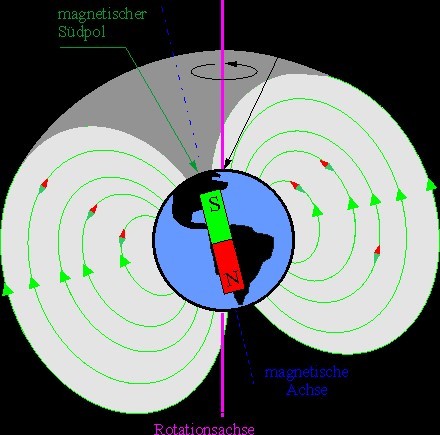
\includegraphics[width=0.50\textwidth]{ref/images/magnetfeld.jpg}
 
Das Erdmagnetfeld ist in Abbildung XX zu sehen. Durch dieses Feld ist die komplette Erdkugel magnetisiert. In der Nähe des geografischen Südpols liegt der magnetische Nordpol. Umgekehrtes gilt für den geografischen und magnetischen Nord- bzw. Südpol.
Damit ein Kompass dieses Feld nutzen kann wird ein magnetisches Metallstück benötigt. Da die magnetische Anziehung nicht sehr stark ist, sollte das Metallstück sehr leichtgängig sein. Hierfür besitzen die meisten Kompasse ein rundes Gehäuse welches mit einer Flüssigkeit gefüllt ist. In dieser Flüssigkeit ist das Metallstück in der Mitte fixiert und kann sich so mit sehr geringem Reibungswiderstand drehen. Hält man den Kompass waagerecht und dreht sich nicht dabei, wird sich das magnetisierte Metallstück Richtung geografischem Nordpol ausrichten. Bei einem Kompass wird dieses Metallstück Nadel genannt und ist meist in den Farben rot und grün lackiert. Die Rote Spitze der Nadel zeigt nach Norden.

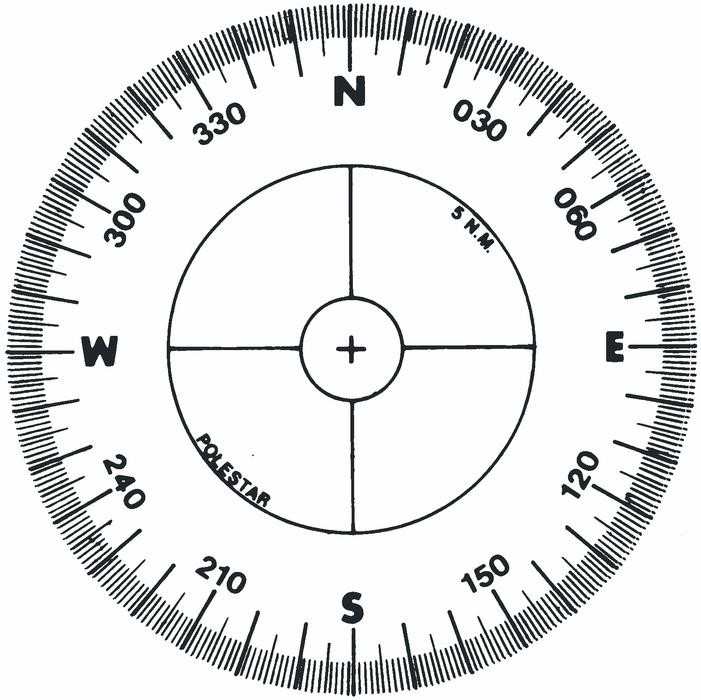
\includegraphics[width=0.50\textwidth]{ref/images/kompassrose.jpg}
 
Bei einem Kompass kommt neben der Nadel auch eine Kompassrose zum Einsatz. Diese ist unter der Nadel angebracht und entweder fest mit dem Gehäuse oder der Nadel verbunden. Mit Hilfe dieser Rose lässt sich eine Gradzahl ablesen diese Gradzahl orientiert sich immer am Abstand von der angezeigten Richtung des Norpols. Diese Gradzahl kann für die Beschreibung des eigenen Standort genutzt werden. Wie dieses Verfahren funktioniert wird im nächsten Abschnitt erklärt.

Standortbeschreibung mit zwei Fixpunkten
Möchte man seinen geografischen Standpunkt jemandem Mitteilen oder sich dieses notieren, muss man diesen beschreiben. Hat man dafür nur einen Kompass zur Verfügung, kann man sich zwei Fixpunkte zur Hilfe nehmen um den eigenen Standort zu bestimmen.
Anhand eines Beispiels soll dieses Verfahren erklärt werden. Befindet man sich auf einem Boot in der Nähe der Küste und möchte den Standort mit einem Kompass bestimmen, so sucht man sich zwei gut sichtbare Punkte an der Küste, dies können beispielsweise Leuchttürme oder eindeutig identifizierbare Felswände sein. Nun fixiert man den ersten Punkt mit dem Kompass. Anschließend liest man die exakte Grad Zahl auf der Kompassrose ab.  In Abbildung XX entspricht dies der blauen Linie (TODO). Mit Hilfe der Angabe von Gradzahl und erstem Fixpunkt, kann der eigene Standort auf eine Linie differenziert werden. Um nun den Standort auf einen Punkt zu differenzieren fixiert man mit dem Kompass den zweiten Fixpunkt und liest ebenfalls die Grad Zahl ab. Zeichnet man diese Informationen in eine Karte ergibt sich ein Schnittpunkt von zwei Geraden. An dieser Stelle befindet man sich. Die Beschreibung des eigenen Standortes könnte beispielsweise wie folgt aussehen:
270 Grad von Leuchtturm X
250 Grad von Gebäude Y
Vorteil, verfahren kann überall angewendet werden wo es fixpunkte Gibt (excl. Offenes Meer)
Nachteile dieser Methode sind, es wird keine Höhe angegeben und es kann eine große Ungenauigkeit beim Ablesen des Kompasses entstehen.

\textbf{Standortbeschreibung mittels einer Adresse}
Im Gegensatz zur eben Vorgestellten Standortbeschreibung ist die in diesem Abschnitt behandelt wird wesentlich bekannte. Es handelt sich um die Anschrift bzw. Adresse. Bei dieser Beschreibung wird kein exakter Standort angeben, sondern ein Haushalt. Dies geschieht über einen Namen, eine Straße mit Hausnummer und die Angabe einer Stadt welche konkretisiert über die Postleitzahl angeben wird.  
Eine Adresse kann in Deutschland beispielsweise wie folgt aus:
Max Mustermann 
Coblitzalle 53
12345 Mannheim

3. Zeile: Postleitzahl und Stadtname
Die letzte Zeile der Adresse enthält den Namen einer Stadt sowie eine Postleitzahl. Bei der Angabe der Stadt handelt es sich um die gröbste Angabe innerhalb der Adresse. Mit Hilfe des Städtenames soll eine erste Orientierung innerhalb deutschlands ermöglicht werden. Es handelt sich nicht nur um Großstädte wie Berlin, Frankfurt, Hamburg etc. sondern alle Gemeinden welche den Titel Stadt tragen .
Da manche Städtenamen mehrfach vorkommen oder die Angabe zu ungenau ist wird der Stadname mit der Postleitzahl (PLZ) definiert bzw. konkretierst. Alleine für die Stadt Mannheim gibt es über 15 verschieden PLZs. Diese sind teilweise jedem Stadtteil zugeordnet.

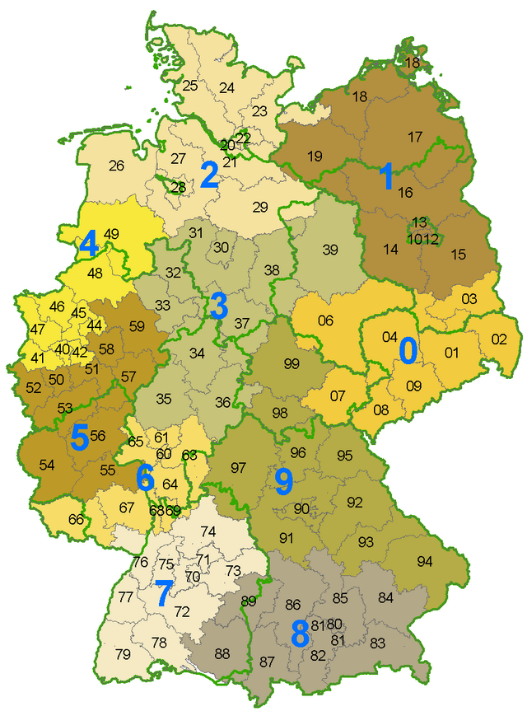
\includegraphics[width=0.50\textwidth]{ref/images/plzgebiete.png}

 Die PLZs in Deutschland haben sich im Laufe der Jahre häufig geändert, seit 1993 gibt es fünfstellige PLZs in Deutschland. Die erste Ziffer 0-9 gibt ein Gebiet an. Mit jeder weiteren Ziffer wird das Gebiet konkretisiert. Siehe Abbildung XX. Da die Angabe von einer Stadt und dazugehörigen PLZ, das Gebiet noch nicht weit genug einschränkt um einzelne Häuser bzw. Haushalte zu identifizieren, wird ein Straßenname angegeben.
Die europäischen Straßennamen sind meist mit Wort Namen angeben.
Einige Beispiele hierfür sind:
-	Lindenstraße
-	Schillerstraße
-	Hauptstraße
Teilweise sind die Namen historisch gewachsen, eine Hauptstraße beispielsweise war früher eine Haupthandelsroute für reisende. Auch Berühmte Persönlichkeiten wie Schriftsteller oder Politiker werden als Straßennamen verwendet. Besonders zu beachten ist, dass eine Straße eindeutig in einem PLZ Gebiet identifiziert werden kann.
Um ein Haus innerhalb einer Straße exakt definieren zu können bedient man sich einer Nummerierung. Den sogenannten Hausnummern. Jedes Haus hat eine eigene Hausnummer. 
In Deutschland findet die Nummerierung der Häuser nach einer speziellen Ordnung statt. Auf einer Straßenseite wird mit der Zahl eins begonnen, auf der anderen Straße bekommt das erste Haus die Nummer zwei. Diese Ordnung wird bis zum Ende der Straße vortgeführt, daraus resultierte, dass eine Straßenseite nur gerade Hausnummern besitzt und die andere nur ungerade.
Da es nicht selten vorkommt, dass in einem Haus mehrere Parteien wohnen, wird neben den Beschriebenen Bestandteilen einer Adresse noch ein Empfänger mit Vor- und Nachname oder nur Nachnahme angegeben.
Diese Beschreibung findet auf der ganzen Welt anwenund, allerdings nicht immer in diesem Format. Das beschrieben Format trifft größtenteils in Europa zu. Zwei Beispiele für die Abweichung dieser Beschreibung, sind die Stadt Mannheim und die vereinigten Staaten von Amerika.
In Mannheim ist die Innenstadt in Quadrate aufgeteilt. Siehe Abbildung XX 

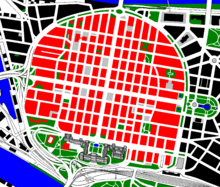
\includegraphics[width=0.50\textwidth]{ref/images/quadratemannheim.png}

Dort gibt es keine Straßennamen sondern nur Koordinaten mit einem Buchstaben und einer Zahl.
!!TODO!! In New York wird eine Straße in realtion zu einem Fixpunkt angegeben. Es wird als Straßenname angebgen die wie vielte Straße es ist vom definierten Fixpunkt !!TODO!! 



Verwendung von Adressen
Die vorgestellte Beschreibung des eigenen Standortes mithilfe einer Adresse ist besonders wichtig für Brief- und Paketversandorganisationen. In Deutschland wurden in den letzten Jahre hauptsächlich mit der Deutschen Post AG Briefe verschickt. Diese ist darauf angewiesen, dass auf jedem Pakte und Brief die Adresse im beschriebenen Format angegeben ist damit eine Zustellung erfolgen kann.
Desweiteren  hat die Adresse stark an Bedeutung dazu gewonnen mit der Entwicklung von Navigationsgeräten. Im Jahr 2014 haben ca. 48% der deutschen Haushalte ein Navigationsgerät besessen. Dort wird das Ziel hauptsächlich als Adresse angegeben. 
Auch im Alltag wird die Adresse meist zur Beschreibung des eigenen Standortes verwendet. Möchte man Freunde zu sich einladen gibt man meist die Adresse an und mit eine Navigationsgerät oder einer Karte kann der Haushalt gefunden werden.
Vergleicht man eine Adresse mit der Standortbeschreibung des letzten Kapitels über einen Kompass ist zu erkennen, dass man sich einen groben Überblick über den Standort mit Adresse viel leichter verschaffen kann. Die Koordinaten eines Kompass kann man nur mit entsprechendem Fachwissen deuten. 
Als Nachteile zählen die Genaugkeit und Abdeckung der Erde mit Adressen. Die Genaugkeit des eigenen Standortes kann mit einer Adresse nicht exakt angegeben werden. Während bei einer kleinen Einzimmerwohnung der Standort auf wenige Meter genau angegeben werden kann, kann sich dies auf mehrere Kilometer ausweiten wenn die Adresse zu einem großen Anwesen gehört. Für manche Location Based Sevices ist es wichtig, dass diese auch in nicht besiedelten Gebieten verwendet werden können. Hierzu zählen Beispielsweise LBS zum Wandern und Radfahren. Hierfür eignet sich die Angabe des eigenen Standortes mit einer Adresse nicht, da ein Standort nur auf der Minderheit der Erde mit einer Adresse angegeben werden kann. 
Im nächsten Abschnitt wird die Beschreibung des Standortes mithilfe von Längen- und Breitengraden erläutert.

\textbf{Standortbeschreibung mit Längen- und Breitengraden}

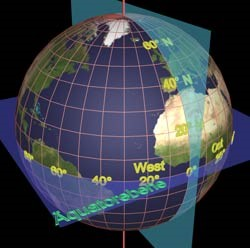
\includegraphics[width=0.50\textwidth]{ref/images/grade.jpg}

Dieser Abschnitt erläutert die Standortbeschreibung mittels Längen- und Breitengrade.
Bildlich kann man sich ein zweidimensionales Koordinatensystem vorstellen, welches den Nullpunkt im Zentrum besitzt, diese „Netz “ legt man bildlich gesprochen über den Globus. So kann für jeden Ort auf dem Globus eine exakte Beschreibung stattfinden. 
Grundlagen für diese Standortbeschreibung
Beim Globus handelt es sich annährend um eine Kugel. Diese Kugel dreht sich in ca. 24 Stunden um ihre eigene Achse. Die Achse kann man sich als gedachte Gerade vorstellen, welche an der untersten Stelle, dem Südpol einsticht und am obersten Punkt wieder austritt, dem Nordpol. Stellt man sich nun die Achse als Strecke von Nord- nach Südpol vor und halbiert diese, befindet man sich im ungefähren Mittelpunkt des Globus. Spannt man auf der Höhe der halbierten Achse einen Kreis um den Globus, so befindet man sich an der dicksten Stelle, dem Äquator. Dieser befindet sich im Rechtenwinkel zur Achse.

Breitengrade
Nachdem der Äquator im letzten Abschnitt definiert wurde, wird nun erklärt was Breitengrade sind. Um den gesamten Globus mit Graden zu beschreiben, hat man sich dazu entschieden den Globus am Äquator in eine nördliche und eine südliche Halbkugel aufzuteilen. Der Gesamte Globus ist in 180 Breitengrade aufgeteilt. Beim Äquator handelt es sich um den 0. Grad. In Abhängigkeit dieses Grades wird der Standort auf einem Längengrad angegeben. Es gibt jeweils 90 Grade in die nördliche und südliche Richtung. Mithilfe dieser Angabe kann man seinen Standort auf eine Linie um den Globus beschränken. Die Stadt Mannheim beispielsweise liegt auf der Linie welche im 49 Grad Winkel zum Äquator steht auf der nördlichen Halbkugel. Im Vergleich hierzu liegt Sydney im 33 Grad Winkel zum Äquator auf der südlichen Halbkugel.
Damit der eigene Standort nicht nur einer Linie beschrieben werden kann, welche im schlimmsten Fall 40.075km lang ist, gibt es Längengrade. Diese Beiden Grade schneiden sich bei der Standortbeschreibung in einem Punkt und geben den Standort exakt an.

Längengrade
Ähnlich wie bei Breitengraden handelt es sich bei Längengraden um gedachte Linien um den Globus. Längengrade stehen allerdings senkrecht zum Äquator und nicht parallel wie die Breitengrade. Bei diesen Graden ist zu beachten, dass sie immer den gleichen Umfang besitzen. Um den kompletten Globus abzudecken gibt es 360 Längengrade. Diese wurden aufgeteilt in westliche und östliche Grade mit jeweils 180 Grad. Für Längengrade gibt es keinen gegebenen Nullpunkt wie den Äquator. 1883 wurde sich darauf geeinigt den Nullmeridian (0 Längengrad) durch eine Sternenwarte im englischen Greenwich laufen zu lassen. Seit dieser Einigung wird wird er Längengrad in Abhängigkeit des Winkels zur Stadt Grennwich angegeben. 
Um auf die Beispiele des letzten Abschnitts zurück zukommen, die Stad Mannheim liegt auf dem 8. Längengrad östlich von Grennwich und Sydney 151. Grad östlich von Greenwich.

Genauigkeit der Längen- und Breitengrade
Der Umfang des Globus beträgt ca. 40.000 km. Teilt man diesen nun durch 360 Längengrade erhält man einen Abstand von 111km zwischen zwei Längengraden. Das bedeutet, wenn der Längengrad  lediglich mit einer Gradzahl angegeben ist, handelt es sich um eine Strecke von 111km auf dem der Standort liegen kann. Daher teilt man entweder ein Grad in 60 Minuten und eine Minute in 60 Sekunden, was eine Strecke von 30m entspricht oder man gibt zu einer Grad Zahl Dezimalstellen an. Bei der Angabe von 5 Dezimalstellen beträgt die Genauigkeit 1 Meter.
Durch die Krümmung der Erde, lässt sich diese Rechnung nicht auf Breitengrade übertragen. 
handelt es sich ca um ein Gebiet von 111 kmhoch2. Dies ist selbstverständlich nicht genau genug um den eigenen Standort zu beschreiben. Deshalb wird ein Grad in 60 Minuten unterteilt. Draus resultiert eine Genauigkeit von 1,85 kmhoch2. Da dies immer noch nicht genau genug ist, teilt man eine Minute in 60 Sekunden. Damit ergibt sich eine Genauigkeit von 30 mhoch2. 


Adresse + PLZ, analoge Karte, Länge+Breit, 3D-Position, indoor (WLAN Blue)